% !TEX program = pdflatex
%!TEX spellcheck
%%
%% This is file `sample-acmsmall-submission.tex',
%% generated with the docstrip utility.
%%
%% The original source files were:
%%
%% samples.dtx  (with options: `acmsmall-submission')
%% 
%% IMPORTANT NOTICE:
%% 
%% For the copyright see the source file.
%% 
%% Any modified versions of this file must be renamed
%% with new filenames distinct from sample-acmsmall-submission.tex.
%% 
%% For distribution of the original source see the terms
%% for copying and modification in the file samples.dtx.
%% 
%% This generated file may be distributed as long as the
%% original source files, as listed above, are part of the
%% same distribution. (The sources need not necessarily be
%% in the same archive or directory.)
%%
%% The first command in your LaTeX source must be the \documentclass command.
\documentclass[acmsmall,screen,review,anonymous]{acmart}

%%
%% \BibTeX command to typeset BibTeX logo in the docs
\AtBeginDocument{%
  \providecommand\BibTeX{{%
    \normalfont B\kern-0.5em{\scshape i\kern-0.25em b}\kern-0.8em\TeX}}}

%% Rights management information.  This information is sent to you
%% when you complete the rights form.  These commands have SAMPLE
%% values in them; it is your responsibility as an author to replace
%% the commands and values with those provided to you when you
%% complete the rights form.
\setcopyright{acmcopyright}
\copyrightyear{2018}
\acmYear{2018}
\acmDOI{10.1145/1122445.1122456}


%%
%% These commands are for a JOURNAL article.
\acmJournal{JACM}
\acmVolume{37}
\acmNumber{4}
\acmArticle{111}
\acmMonth{8}

%%
%% Submission ID.
%% Use this when submitting an article to a sponsored event. You'll
%% receive a unique submission ID from the organizers
%% of the event, and this ID should be used as the parameter to this command.
%%\acmSubmissionID{123-A56-BU3}

%%
%% The majority of ACM publications use numbered citations and
%% references.  The command \citestyle{authoryear} switches to the
%% "author year" style.
%%
%% If you are preparing content for an event
%% sponsored by ACM SIGGRAPH, you must use the "author year" style of
%% citations and references.
%% Uncommenting
%% the next command will enable that style.
%%\citestyle{acmauthoryear}

%% Bibliography style
\bibliographystyle{ACM-Reference-Format}
%% Citation style
%\citestyle{acmauthoryear}  %% For author/year citations
%\citestyle{acmnumeric}     %% For numeric citations
%\setcitestyle{nosort}      %% With 'acmnumeric', to disable automatic
                            %% sorting of references within a single citation;
                            %% e.g., \cite{Smith99,Carpenter05,Baker12}
                            %% rendered as [14,5,2] rather than [2,5,14].
%\setcitesyle{nocompress}   %% With 'acmnumeric', to disable automatic
                            %% compression of sequential references within a
                            %% single citation;
                            %% e.g., \cite{Baker12,Baker14,Baker16}
                            %% rendered as [2,3,4] rather than [2-4].


%%%%%%%%%%%%%%%%%%%%%%%%%%%%%%%%%%%%%%%%%%%%%%%%%%%%%%%%%%%%%%%%%%%%%%
%% Note: Authors migrating a paper from traditional SIGPLAN
%% proceedings format to PACMPL format must update the
%% '\documentclass' and topmatter commands above; see
%% 'acmart-pacmpl-template.tex'.
%%%%%%%%%%%%%%%%%%%%%%%%%%%%%%%%%%%%%%%%%%%%%%%%%%%%%%%%%%%%%%%%%%%%%%


%% Some recommended packages.
\usepackage{booktabs}   %% For formal tables:
                        %% http://ctan.org/pkg/booktabs
\usepackage{subcaption} %% For complex figures with subfigures/subcaptions
                        %% http://ctan.org/pkg/subcaption

\usepackage{algorithm}
\usepackage{tabularx}
\usepackage{algorithmic}
\usepackage{proof}
\usepackage{alltt}
\usepackage{pgf}
\usepackage{bcproof}
\usepackage{setspace}

\renewcommand{\algorithmicrequire}{\textbf{Input:}}

\renewcommand{\algorithmicensure}{\textbf{Output:}}

\newtheorem{Def}{Definition}[section]
\newtheorem{mythm}{Theorem}[section]
\newtheorem{property}{Property}[section]
\newtheorem{lemma}{Lemma}[section]
\newtheorem{Asm}{Assumption}

\newcommand{\Code}[1]{\texttt{#1}}
\newenvironment{Codes}
  {\begin{alltt}\leftskip=1.5em} % \tiny
  {\end{alltt}}

\newenvironment{smallCodes}
  {\begin{alltt}\leftskip=1.5em\small} %
  {\end{alltt}}

\newcommand{\OneStep}{{\rule{0pt}{1.2\baselineskip}{\ensuremath\longrightarrow}}}
\newcommand{\DeStep}{{\rule{0pt}{1.2\baselineskip}{\ensuremath\dashrightarrow}}}

\newcommand\m[1]{\mbox{\tt #1}}
\newcommand\key[1]{\mbox{\rm \bf #1}}
\newcommand\drule[2]{#1 ~\rightarrow_d~ #2}
\newcommand\redc[2]{#1 ~\rightarrow_c~#2}
\newcommand\rede[2]{#1 ~\rightarrow_e~#2}
\newcommand\redm[2]{#1 ~\rightarrow_m~#2}
\newcommand\note[1]{\mbox{{\scriptsize #1}}}
\newcommand\ignore[1]{}

\def\coreId{\m{cId}}
\def\surfId{\m{sId}}
\def\headId{\m{hId}}

\def\true{\#t}
\def\false{\#f}

\def\myend{\flushright{\qed}}

% some macros for editing/commenting the paper

\def\modify#1#2#3{{\small\underline{\sf{#1}}:} {\color{red}{\small #2}}
{{\color{red}\mbox{$\Rightarrow$}}} {\color{blue}{#3}}}

\newcommand{\hmodify}[2]{\modify{Hu}{#1}{#2}}
\newcommand\mymargin[1]{\marginpar{{\flushleft\textsc\footnotesize {#1}}}}
\newcommand\hmargin[1]{\mymargin{Hu:\;#1}}

\newcommand{\hmodifyok}[2]{#2}

\newcommand{\mycomment}[2]{{\small\color{magenta}\underline{\sf{#1}}:} {\color{magenta}{\small #2}}}
\newcommand{\hcomment}[1]{\mycomment{Hu}{#1}}
\newcommand{\gcomment}[1]{\mycomment{G}{#1}}
\newcommand{\todo}[1]{\mycomment{Todo}{#1}}

\newcommand{\xcomment}[1]{\mycomment{X}{#1}}
\newcommand{\ycomment}[1]{\mycomment{Y}{#1}}

\newcommand{\reduce}[1]{{\color{blue}{#1}}}
\newcommand{\reducedversion}[1]{{\color{blue}{#1}}}

\newcommand{\example}[3]{
\begin{figure}[thb]
\begin{center}
#1
\end{center}
\caption{#2}
\label{#3}
\end{figure}
}

\makeatletter
\newcommand{\xleftrightarrow}[2][]{\ext@arrow 3359\leftrightarrowfill@{#1}{#2}}
\newcommand{\xdashrightarrow}[2][]{\ext@arrow 0359\rightarrowfill@@{#1}{#2}}
\newcommand{\xdashleftarrow}[2][]{\ext@arrow 3095\leftarrowfill@@{#1}{#2}}
\newcommand{\xdashleftrightarrow}[2][]{\ext@arrow 3359\leftrightarrowfill@@{#1}{#2}}
\def\rightarrowfill@@{\arrowfill@@\relax\relbar\rightarrow}
\def\leftarrowfill@@{\arrowfill@@\leftarrow\relbar\relax}
\def\leftrightarrowfill@@{\arrowfill@@\leftarrow\relbar\rightarrow}
\def\arrowfill@@#1#2#3#4{%
  $\m@th\thickmuskip0mu\medmuskip\thickmuskip\thinmuskip\thickmuskip
   \relax#4#1
   \xleaders\hbox{$#4#2$}\hfill
   #3$%
}
\makeatother

\makeatletter
\newcommand*{\dashdownarrow}{%
  \mathrel{%
    \mathpalette\dasharrow@vert{-90}%
  }%
}
\newcommand*{\dashuparrow}{%
  \mathrel{%
    \mathpalette\dasharrow@vert{90}%
  }%
}
\newcommand*{\dasharrow@vert}[2]{%
  \sbox0{$#1\vcenter{}$}%
  \sbox2{$#1\dashrightarrow\m@th$}%
  \dimen@=1.2\dimexpr\ht2-\ht0\relax
  % 1/2 width of the new symbol with side bearing
  \sbox2{\raisebox{-\ht0}{\unhcopy2}}%
  \ht2=\z@
  \dp2=\z@
  \vcenter{\hbox to 2\dimen@{\hfill\rotatebox{#2}{\box2}\hfill}}%
}
\makeatother

\makeatletter
\newcommand*\bigcdot{\mathpalette\bigcdot@{.5}}
\newcommand*\bigcdot@[2]{\mathbin{\vcenter{\hbox{\scalebox{#2}{$\m@th#1\bullet$}}}}}
\makeatother

\begin{document}

%% Title information
\title{Resugaring by Lazy Desugaring}         %% [Short Title] is optional;
                                        %% when present, will be used in
                                        %% header instead of Full Title.
% \titlenote{with title note}             %% \titlenote is optional;
%                                         %% can be repeated if necessary;
%                                         %% contents suppressed with 'anonymous'
% \subtitle{Subtitle}                     %% \subtitle is optional
% \subtitlenote{with subtitle note}       %% \subtitlenote is optional;
%                                         %% can be repeated if necessary;
%                                         %% contents suppressed with 'anonymous'


%% Author information
%% Contents and number of authors suppressed with 'anonymous'.
%% Each author should be introduced by \author, followed by
%% \authornote (optional), \orcid (optional), \affiliation, and
%% \email.
%% An author may have multiple affiliations and/or emails; repeat the
%% appropriate command.
%% Many elements are not rendered, but should be provided for metadata
%% extraction tools.

\author{anonymous}
\email{@}

%% Abstract
%% Note: \begin{abstract}...\end{abstract} environment must come
%% before \maketitle command
\begin{abstract}


% Syntactic sugar, first coined by Peter J. Landin in 1964, has proved to be very useful for defining domain-specific languages and extending languages. Unfortunately, when syntactic sugar is eliminated by transformation, it obscures the relationship between the user’s source program and the transformed program. Resugaring is a powerful technique to resolve this problem, which automatically converts the evaluation sequences of desugared program in the core language into representative sugar's syntax in the surface language. However, the existing approach relies on the reverse application of desugaring rules to desugared core expression whenever possible. When a desugaring rule is complex and a desugared program is large, such reverse expansion becomes very complex and costive.

% In this paper,
We propose a novel approach to resugaring, which can automatically convert the evaluation sequences of desugared program in the core language into representative sugar's syntax in the surface language by lazy desugaring.
%which  is a technique to get the surface evaluation sequences of syntactic sugars, by lazy desugaring.
We define lazy desugaring by proposing a reduction strategy for the language combining the surface language with the core language, prove that it will produce correct resugaring evaluation sequences, and demonstrate that it is powerful enough to deal with hygienic, recursive and higher-order sugars.
We have implemented a resugaring system based on this new approach, and the experimental results show that our approach is more efficient and powerful than the existing ones.

\end{abstract}


%% 2012 ACM Computing Classification System (CSS) concepts
%% Generate at 'http://dl.acm.org/ccs/ccs.cfm'.
\begin{CCSXML}
<ccs2012>
<concept>
<concept_id>10011007.10011006.10011008</concept_id>
<concept_desc>Software and its engineering~General programming languages</concept_desc>
<concept_significance>500</concept_significance>
</concept>
<concept>
<concept_id>10003456.10003457.10003521.10003525</concept_id>
<concept_desc>Social and professional topics~History of programming languages</concept_desc>
<concept_significance>300</concept_significance>
</concept>
</ccs2012>
\end{CCSXML}

\ccsdesc[500]{Software and its engineering~General programming languages}
\ccsdesc[300]{Social and professional topics~History of programming languages}
%% End of generated code


%% Keywords
%% comma separated list
\keywords{Resugaring, Syntactic Sugar, Domain-Specific Language, Reduction Semantics, Metaprogramming}  %% \keywords are mandatory in final camera-ready submission


%% \maketitle
%% Note: \maketitle command must come after title commands, author
%% commands, abstract environment, Computing Classification System
%% environment and commands, and keywords command.
\maketitle

\todo{
  (1)new sugar form? (full desugared)
}
%!TEX root = ./main.tex
\section{Introduction}

%What is the research background and and what motivate you to do this research?

%What is the research issue and how the issue has been addressed so far?

%What is the remained research problem and how challenge it is?

%What is your key idea (insight) of your solution to be discussed in this paper?

%What are the three main technical contributions of this paper?

%The rest of the paper is organized as follows. ...

Domain-specific language\cite{dsl} is becoming useful for people's daily tasks. For example, the IFTTT app and IOS's shortcuts designed DSLs describing some tasks to make our lives more convenient. So the users of DSL are no longer limited to programmers, but people from all walks of life.(to be completed)

Syntactic sugar\cite{syntacticsugar}, as a simple ways design DSL, has a obvious problem. DSL based on syntactic sugars contains many components of its host language. Then its interpretation will be outside the DSL itself. The evaluation sequences of syntactic sugar expression will contain many terms of the host language, which may confuse the users of DSL.

There is an existing work---resugaring\cite{resugaring}\cite{hygienic}, which aimed to solve the problem upon. It lifts the evaluation sequences of desugared expression to sugar's syntax. The evaluation sequences shown by resugaring will not contain components of host language. But we found the resugaring method using match and substitution is kind of redundant. The biggest deficiency of existing resugaring method is that the syntactic sugars in an expression have to fully desugar before evaluation. This limits the processing ability of the method. Moreover, it limits the complexity of getting the resugaring sequences. If we need to resugar a very huge expression, the match and substitution processes will cost so much. Also, processing of hygienic macros is complex due to the extra data structure.

In this paper, We propose a lightweight approach to get resugaring sequences based on syntactic sugars. The key idea of our approach is---syntactic sugar expression only desugars at the point that it have to desugar. We guess that we don't have to desugar the whole expression at the initial time of evaluation under the premise of keeping the properties of expression. 

Initially, our work focused on improving current resugaring method. After finishing that, we found our lightweight resugaring approach could process some syntactic sugars' feature that current approach cannot do. Finally, we implement our algorithm using PLT Redex\cite{SEwPR} and test our approach on some applications. The result shows that our approach does handle more features of syntactic sugar.

In the rest of this paper, we present the technical details of our approach together with the proof of correctness. In details, the rest of our paper is organized as follow:

\begin{itemize}
\item An overview of our approach with some background knowledge.[sec \ref{sec2}]
\item The algorithm defination and proof of correctness.[sec \ref{sec3}]
\item The implementation of our lightweight resugaring algorithm using PLT Redex.[sec \ref{sec4}]
\item sth else?[sec \ref{sec5}]
\item Evaluation of our lightweight resugaring approach.[sec \ref{sec6}]
\end{itemize}

%!TEX root = ./main.tex
\section{Overview}
\label{sec2}


In this section, we give a brief overview of our approach. To be concrete, we will consider the following simple core language, defining boolean expressions using the \m{if} construct:
\[
\begin{array}{lllll}
e &::=& \m{CoreExp}\\
\m{CoreExp} &::=& \Code{(if~$e$~$e$~$e$)} &\note{// if construct}\\
& |& \true  & \note{// true value}\\
& |& \false & \note{// false value}
\end{array}
\]
The semantics of the language is simple, consisting of the following context rule to specify the computational order:
\[
\begin{array}{lcl}
C &:=& \Code{(if C $e$ $e$)}\\
&|&[\bigcdot] \qquad \note{//evaluation context's hole}\\
\end{array}
\]
and two reduction rules (the letter c means core):
\[
\centering
 \redc{(\m{if}~\true~e_1~e_2)}{e_1}  \qquad \redc{(\m{if}~\false~e_1~e_2)}{e_2}
\]
Assume that our surface language is defined by two syntactic sugars defined by:
%---\emph{and} sugar and \emph{or} sugar on the core language.
\[
\begin{array}{c}
\drule{(\m{And}~e_1~e_2)}{(\m{if}~e_1~e_2~\false)}\\
\drule{(\m{Or}~e_1~e_2)}{(\m{if}~e_1~\true~e_2)}
\end{array}
\]
Now let us demonstrate how to execute \Code{(And (Or \true~\false) (And \false ~\true))}, and get the following resugaring sequence by our approach.
{\small
\begin{Codes}
    (And (Or \true \false) (And \false \true))
\OneStep{ (And \true (And \false \true))}
\OneStep{ (And \false \true)}
\OneStep{ #f}
\end{Codes}
}

Our new resugaring approach eliminates costive "reverse desugaring" by "lazy desugaring", where a syntactic sugar will be expanded only when it is necessary. It consists of following three steps.

{\em Step 1: Calculating Context Rules for Sugars.}
While giving the evaluation rules of the core language, we can derive the following context rules of the surface language.
\[
\begin{array}{lcl}
C &:=& (\m{And}~C~e)\\
&|& (\m{Or}~C~e)\\
&|&[\bigcdot]\\
\end{array}
\]
From the context rules of \m{if}, we can find that the condition ($e_1$) is always evaluated first. Therefore, for expression \Code{(And $e_1$ $e_2$)} defined by syntactic sugar, $e_1$ is also evaluated first, which is the context rule of \m{And}. Similarly, we can calculate the context rule of \m{Or}.

{\em Step 2: Deriving Reduction Rules for the Mixed Language.}
We mix the surface language with the core language as in Fig. \ref{fig:mixexample}, where \m{CommonExp} means the expressions used in both the surface language and the core language both, and derive $\to_m$, a one-step reduction in our mixed language, from the the reduction rules of fhe core language and the given desugaring rules. By using $\to_m$, we can get the following evaluation sequence in the mixed language for
the program \Code{(And (Or \true~\false) (And \false~\true))}

{\footnotesize
\begin{Codes}
    (And (Or \true \false) (And \false \true))
\OneStep{ (And (if \true \true \false) (And \false \true))}
\OneStep{ (And \true (And \false \true))}
\OneStep{ (if \true (And \false \true) \false)}
\OneStep{ (And \false \true)}
\OneStep{ (if \false \true \false)}
\OneStep{ \false}
\end{Codes}
}


\begin{figure}[t]
\centering
\begin{subfigure}{\linewidth}{\footnotesize
    \begin{flushleft}
        \[
        \begin{array}{lll}
        e &::=& \m{CoreExp} \\
        &|&\m{SurfExp}\\
        &|&\m{CommonExp}\\
        \m{CoreExp} &::=& \Code{(if~$e$~$e$~$e$)}\\
        \m{SurfExp} &::=& \Code{(And~$e$~$e$)}\\
        &|&\Code{(Or~$e$~$e$)}\\
        \m{CommonExp} &::=& \true\\
        &|& \false\\
        \end{array}
        \]
    \end{flushleft}
    \caption{Syntax}
    \label{fig:mixsyntax}
}
\end{subfigure}
\begin{subfigure}{\linewidth}{\footnotesize
    \begin{flushleft}
        \[\footnotesize
        \begin{array}{lcl}
        C &:=& (\m{if}~C~$e$~$e$)\\
        &|& (\m{And}~C~$e$)\\
        &|& (\m{Or}~C~$e$)\\
        &|&[\bigcdot]\\
        \end{array}
        \]
        \end{flushleft}
    \caption{Context Rules}
    \label{fig:mixcontext}
}
\end{subfigure}

\begin{subfigure}{\linewidth}{\footnotesize
    \begin{flushleft}
        \[
        \begin{array}{c}
        \redm{(\m{And}~e_1~e_2)}{(\m{if}~e_1~e_2~\false)}\\
        \redm{(\m{Or}~e_1~e_2)}{(\m{if}~e_1~\true~e_2)}\\
        \redm{(\m{if}~\true~e_1~e_2)}{e_1}\\
        \redm{(\m{if}~\false~e_1~e_2)}{e_2}
        \end{array}
        \]
    \end{flushleft}
    \caption{Reduction Rules}
    \label{fig:mixreduction}
}
\end{subfigure}

\caption{Mixed Language Example}
\label{fig:mixexample}
\end{figure}


{\em Step 3: Removing Unnecessary Expressions.}
We can just keep the intermediate sequences without \m{Coreexp} in any sub-expressions to get the resugaring sequence above.

%Note that the context rules should restrict the computational order of a sugar expression's sub-expressions, thus we should let the context rules be correct---reflecting what should be executed in the desugared expression.
Note that as the goal of resugaring is to present the evaluation of sugar programs, we are given a way to clearly specify which expression should be outputted. For the example in this section, of course, the sugar \m{And} and \m{Or} should be outputted, and also the boolean values should be. So we set boolean values as \m{CommonExp} in Fig. \ref{fig:mixsyntax}, so that they can be displayed though they are in the core language. By clearly separating what should be displayed, we can always get the resugaring evaluation sequences we need (this is slightly different from the existing approach's setting, as we will discuss in Section \ref{mark:correctness}.)

%!TEX root = ./main.tex

\section{Resugaring by Lazy Desugaring}
\label{sec3}

In this section, we present our new approach to resugaring. Different from the traditional approach that clearly separates the surface and the core languages, we combine them together as one mixed language, allowing users to freely use the language constructs in both languages. We will show that any expression in the mixed language can be evaluated in such a smart way that a sequence of all expressions that are necessarily to be resugared by the traditional approach can be correctly produced.

\subsection{Mixed Language for Resugaring}

\begin{figure}[t]
	\[
	\begin{array}{lllll}
	 &\m{CoreExp} &::=& x  & \note{variable}\\
	       &&~|~& c  & \note{constant}\\
				 &&~|~& (\m{CoreHead}~\m{CoreExp}_1~\ldots~\m{CoreExp}_n) & \note{constructor}\\
	\\
	 &\m{SurfExp} &::=& x  & \note{variable}\\
	       &&~|~& c  & \note{constant}\\
				 &&~|~& (\m{CoreHead}~\m{SurfExp}_1~\ldots~\m{SurfExp}_n) & \note{selected core constructor}\\
					 &&~|~& (\m{SurfHead}~\m{SurfExp}_1~\ldots~\m{SurfExp}_n) & \note{sugar expression}\\
	\end{array}
	\]
	\caption{Core and Surface Expressions}
	\label{fig:expression}
\end{figure}

We will define a mixed language for a given core language and a surface language defined over the core language. An expression in this language will be reduced step by step by the reduction rules for the core language and the desugaring rules for defining the syntactic sugars in the surface language.

\subsubsection{Core Language}

For our host language, we consider its evaluator as a blackbox \todo{need to be corrected.} but with two natural assumptions. First, there is a deterministic stepper in the evaluator which, given an expression in the host language, can deterministically reduce the expression to a new expression. Second, the evaluation of any sub-expression has no side-effect on other parts of the whole expression.

An expression of the core language is defined in Figure \ref{fig:expression}. It is a variable, a constant, or a (language) constructor expression. Here, $\m{CoreHead}$ stands for a language constructor such as $\m{if}$ and $\m{let}$. To be concrete, we will use the core language defined in Figure \ref{fig:core} to demonstrate our approach.

\begin{figure}[t]
\begin{center}
\begin{tabularx}{.9\textwidth}%
{|>{\setlength{\hsize}{.4\hsize}\centering\arraybackslash}X  |>{\setlength{\hsize}{1.6\hsize}\centering\arraybackslash}X|}
%{|*{2}{>{\centering\arraybackslash}X|}}
\hline
Syntax & Reduction rules \\ \hline
(if e e e) &\qquad\qquad\qquad(if \#t e2 e3) $\rightarrow$ e2 \newline ~(if \#f e2 e3) $\rightarrow$ e3\\ \hline
(($\lambda$ (x ...) e) e ...) & (($\lambda$ (x0 x1 ...) e) v0 v1 ...) $\rightarrow$ (let ((x0 v0) (($\lambda$ (x1 ...) e) v1 ...))\\ \hline
(($\lambda_N$ (x ...) e) e ...) & (($\lambda_N$ (x0 x1 ...) e) e0 e1 ...) $\rightarrow$ (let ((x0 e0) (($\lambda_N$ (x1 ...) e) e1 ...))\\ \hline
(let ((x e) ...) e) & (let ((x0 e0) (x1 e1) ...) e) $\rightarrow$ (let ((x1 e1) ...) (subst x0 e0 e))\newline (let () e)  $\rightarrow$ e (where subst is a meta function)\\ \hline
(first e) & (first (list v1 v2 ...)) $\rightarrow$ v1\\ \hline
(rest e) & (rest (list v1 v2 ...)) $\rightarrow$ (list v2 ...)\\ \hline
(empty e) & \qquad\qquad\qquad(empty (list)) $\rightarrow$ \#t \newline (empty (list v1 ...)) $\rightarrow$ \#f\\ \hline
(cons e e) & (cons v1 (list v2 ...)) $\rightarrow$ (list v1 v2 ...)\\ \hline
(op e e) \newline op=+-*/><== & (op v1 v2) $\rightarrow$ arithmetic result\\ \hline
\end{tabularx}
\end{center}
\caption{An Core Language Example}
\label{fig:core}
\end{figure}


%For simplicity, we use the prefix notation. For instance, we write $\m{if-then-else}~e_1~e_2~e_3$, which would be more readable if we write $\m{if}~e_1~\m{then}~e_2~\m{else}~e_3$. In this paper, we may write both if it is clear from the context.

\subsubsection{Surface Language}

Our surface language is defined by a set of syntactic sugars, together with some language constructs in the core language. So an expression of the surface language is some core constructor expressions with sugar expressions, as defined in Figure \ref{fig:expression}.

A syntactic sugar is defined by a desugaring rule in the following form:
\[
\drule{(\m{SurfHead}~x_1~x_2~\ldots~x_n)}{\m{SurfExp}}
\]
where its LHS is a simple pattern (unnested) and its RHS is a surface expression. For instance, we may define syntactic sugar \m{And} by
\[
\drule{(\m{And}~x~y)}{\m{if}~x~y~\false}.
\]
Note that if the pattern is nested, we can introduce a new syntactic sugar to flatten it.
One may wonder why not restricting the RHS to be a core expression $\m{CoreExp}$, which sounds more natural. We use $\m{surfExp}$ to be able to allow definition of recursive syntactic sugars, as seen in the following example.
\[
\begin{array}{l}
\drule{(\m{Odd}~x)}{\m{if}~(>~x~0)~(\m{Even}~(−~x~1))~\false)}\\
\drule{(\m{Odd}~x)}{\m{if}~(>~x~0)~(\m{Odd}~(−~x~1))~\true)}
\end{array}
\]

We assume that all desugaring rules are not overlapped in the sense that for a syntactic sugar expression, only one desugaring rule is applicable.

\ignore{
\subsubsection{Grammatical restrictions}
Firstly, the whole language should be restricted to tree-structured disjoint expression.

\begin{Def}[disjoint]
For every sub-expression in a expression, its reduction rule is decided by itself.
\end{Def}

This restriction limits the scope of language. Every sub-expression must have no side effect. We will discuss more on side effect in ...

\begin{Def}[tree-structured]
The grammar of the whole language is defined as follow.
\[
\begin{array}{rcl}
\mbox{Exp} &::=& (\mbox{Headid}~\mbox{Exp}*)\\
&|& \mbox{Value}\\
&|& \mbox{Variable}
\end{array}
\]
\end{Def}

The grammatical restrictions give our language a similiar property as church-rosser theorem for lambda calculus.

todo:church-rosser?

\subsubsection{Context restrictions}
For expressions in CoreLang, the context rules should restrict it to have only one reduction path. The context rules can limit the order of evaluation. This restriction is normal, because a program in general-purposed language should have only one execution path.\label{mark:ctx}

For expressions in SurfLang, context rules should allow every sub-expressions reduced. It's the same as full-$\beta$ reduction.

\subsubsection{Restriction of syntactic sugar}
The form of syntactic sugar is as follow.

\fbox{
$(\mbox{Surfid}\;e_{1}\;e_{2}\;\ldots)$ ~→~ $(\mbox{Headid}\; \ldots)$
}

An counter example of this restriction is $(\mbox{Surfid}\;\ldots\;(e1\;e2)\ldots))$ in LHS. It's for simpler algorithm form, and the expression ability of syntactic sugar will not be changed.

\begin{Def}[Unambiguous]
For every syntactic sugar expressions, it can only desugar to one expression in CoreLang.
\end{Def}

}

\subsubsection{Mixed Language}

\begin{figure}[t]
\begin{centering}
	\framebox[36em][c]{
		\parbox[t]{33em}{
			\[
			\begin{array}{lcl}
			\m{Exp} &::=& \m{DisplayableExp}\\
			&|& \m{UndisplayableExp}\\
\\
			\m{DisplayableExp} &::=& \m{SurfExp}\\
			&|& \m{CommonExp}
\\
			\m{UndisplayableExp} &::=& \m{CoreExp}\\
			&|& \m{OtherSurfExp}\\
			&|& \m{OtherCommonExp}\\
\\
			\m{CoreExp} &::=& (\m{CoreHead}~\m{Exp}*)\\
\\
			\m{SurfExp} &::=& (\m{SurfHead}~\m{DisplayableExp}*)\\
\\
			\m{CommonExp} &::=& (\m{CommonHead}~\m{DisplayableExp}*)\\
			&|& c \qquad \note{// constant value}\\
			&|& x \qquad \note{// variable} \\
\\
			\m{OtherSurfExp} &::=& (\m{SurfHead}~\m{Exp}*~\m{UndisplayableExp}~\m{Exp}*)\\
\\
			\m{OtherCommonExp} &::=& (\m{CommonHead}~\m{Exp}*~\m{UndisplayableExp}~\m{Exp}*)
			\end{array}
			\]
		}
	}
\end{centering}
\caption{Our Mixed Language}
\label{fig:mix}
\end{figure}

Our mixed language for resugaring combines the surface language and the core language.
%
The difference between our core language (CoreLang) and our surface language (SurfLang) is identified by $\m{HeadId}$. But there are some terms in the core language should be displayed during evaluation, or we need some terms to help us getting better resugaring sequences. So we defined \m{CommonExp}, which origin from CoreLang, but can be displayed in resugaring sequences. The \m{CoreExp} terms are terms with undisplayable CoreLang's \m{Headid}. The \m{SurfExp} terms are terms with SurfLang's \m{Headid} and all sub-expressions are displayable. The \m{CommonExp} terms are terms with displayable CoreLang's Headid, together with displayable sub-expressions. There exists some other expression during our resugaring process, which have \m{Headid} which can be displayed, but one or more subexpressions cannot. They are \m{UndisplayableExp}.
\todo{Do we need \m{HeadId}?}

Take some terms in the core language in Figure \ref{fig:core} as examples.
We may assume \m{if}, \m{let}, \m{$\lambda _{N}$}, \m{empty}, \m{first}, \m{rest} as \m{CoreExp}'s \m{Headid}, \m{op}, \m{$\lambda$}, \m{cons} as \m{CommonExp}'s \m{Headid}. Then we could show some useful intermediate steps.


\subsection{Resugaring Algorithm}

Our resugaring algorithm works on our mixed language, based on the reduction rules of the core language and the desugaring rules for defining the surface language. Let $\redc{}{}$ denote a one-step reduction of the core language, and $\drule{}{}$ a one-step desugaring by a desuaring rule. We define $\redm{}{}$, a one-step reduction of our mixed language, as follows.

\infrule[CoreRed]
{\redc{(\m{CoreHead}~e_1~\ldots~e_n)}{e'}}
{\redm{(\m{CoreHead}~e_1~\ldots~e_n)}{e'}}

\infrule[SurfaceRed]
{\drule{(\m{SurfHead}~x_1~\ldots~x_i~\ldots~x_n)}{e}\\
 \redm{e[e_1/x,\ldots,e_i/x_i,\ldots,e_n/x_n]}{e[e_1/x,\ldots,e_i'/x_i,\ldots,e_n/x_n]}
}
{\redm{(\m{SurfHead}~e_1~\ldots~e_i~\ldots~e_n)}{(\m{SurfHead}~e_1~\ldots~e_i'~\ldots~e_n)}}


Our resugaring algorithm is based on a core algorithm f. For every expression during resugaring process, it may have one or more reduction rules. The core algorithm f chooses the one that satisfies three properties of resugaring, then applies it on the given expression. The core algorithm f is defined as \ref{alg:f}.
\begin{algorithm}
	\caption{Core-algorithm f}
	\label{alg:f}     % 给算法一个标签,以便其它地方引用该算法
	\begin{algorithmic}[1]       % 数字 "1" 表示为算法显示行号的时候,每几行显示一个行号,如:"1" 表示每行都显示行号,"2" 表示每两行显示一个行号,也是为了方便其它地方的引用
		\REQUIRE ~~\\      % 算法的输入参数说明部分
		Any expression $Exp$=$(Headid~Subexp_{1}~\ldots~Subexp_{\ldots})$ which satisfies Language setting
		\ENSURE ~~\\     % 算法的输出说明
		$Exp'$ reduced from $Exp$, s.t. the reduction satisfies three properties of resugaring
		\STATE     Let $ListofExp'$ = $\{Exp'_{1}\;,Exp'_{2}~\ldots\}$
		\IF {$Exp$ is Coreexp or  Commonexp or OtherCommonexp}
		\IF {Lengthof($ListofExp'$)==0}
		\RETURN null; \hfill Case1
		\ELSIF {Lengthof($ListofExp'$)==1}
		\RETURN first($ListofExp'$); \hfill Case2
		\ELSE
		\RETURN $Exp'_{i}$ = $(Headid~Subexp_{1}~\ldots~Subexp'_{i}~\ldots)$; //where i is the index of subexp which have to be reduced. \hfill Case3
		\ENDIF
		\ELSE
		\IF {$Exp$ have to be desugared}
		\RETURN desugarsurf($Exp$); \hfill Case4
		\ELSE
		\STATE Let $DesugarExp$ = desugarsurf(Exp)
		\IF {$Subexp_{i}$ is reduced to $Subexp'_{i}$ during $f(DesugarExp)$}
		\RETURN $Exp'_{i}$ = $(Headid~Subexp_{1}~\ldots~Subexp'_{i}~\ldots)$; \hfill Case5
		\ELSE
		\RETURN $DesugarExp$; \hfill Case6
		\ENDIF
		\ENDIF
		\ENDIF

	\end{algorithmic}
\end{algorithm}

We briefly describe the core algorithm f in words.

For Exp in language defined as last section, try all reduction rules in the language, get a list of possible expressions ListofExp'=\{$Exp'_{1}$,$Exp'_{2}$,$\ldots$\}.

Line 2-9 deal with the case when Exp has a CoreLang's Headid. When Exp is value or variable (line 3-4), ListofExp' won't have any element (not reducible). When Exp is of Coreexp or Commonexp (line 5-6), due to the context restriction of CoreLang, only one reduction rule can be applied. When Exp is OtherCommonexp (line 7-8), due to the context restriction of CoreLang, only one sub-expression can be reduced, then just apply core algorithm recursively on the sub-expression.

Line 10-21 deal with the case then Exp has a SurfLang's Headid. When Exp only has one reduction rule (line 11-12), the syntactic sugar has to desugar. If not, we should expand outermost sugar and find the sub-expression which should be reduced (line 14-16), or the sugar has to desugar (line 17-18), because it will never be resugared. The steps in line 14 to 16 are the critical part of our algorithm (call {\bfseries one-step try}\label{mark:onesteptry}).


Then, our lightweight-resugaring algorithm is defined as \ref{alg:lwresugar}.

\begin{algorithm}
	\caption{Lightweight-resugaring}
	\label{alg:lwresugar}     % 给算法一个标签,以便其它地方引用该算法
	\begin{algorithmic}[1]       % 数字 "1" 表示为算法显示行号的时候,每几行显示一个行号,如:"1" 表示每行都显示行号,"2" 表示每两行显示一个行号,也是为了方便其它地方的引用
		\REQUIRE ~~\\      % 算法的输入参数说明部分
		Surfexp $Exp$
		\ENSURE ~~\\     % 算法的输出说明
		$Exp$'s evaluation sequences within DSL
		\WHILE {$tmpExp$ = f($Exp$)}
		\IF {$tmpExp$ is empty}
		\RETURN
		\ELSIF {$tmpExp$ is Surfexp or Commonexp}
		\PRINT $tmpExp$;
		\STATE Lightweight-resugaring($tmpExp$);
		\ELSE
		\STATE Lightweight-resugaring($tmpExp$);
		\ENDIF
		\ENDWHILE

	\end{algorithmic}
\end{algorithm}

The whole process of the lightweight resugaring executes core algorithm f, and output sequences which is of Surfexp or Commonexp.

\subsection{Proof of correctness}

First of all, because the difference between our lightweight resugaring algorithm and the existing one is that we only desugar the syntactic sugar when needed, and in the existing approach, all syntactic sugar desugars firstly and then executes on CoreLang.

Second, to prove convenience, define some terms.

$Exp~=~(Headid\;Subexp_{1}\;Subexp_{\ldots} \ldots)$ is any reducible expression in our language.

If we use the reduction rule that desugar Exp's outermost syntactic sugar, then the reduction process is called {\bfseries Outer Reduction}.

If the reduction rule we use reduce $Subexp_{i}$, where $Subexp_{i}$ is $(Headid_{i}~Subexp_{i1}~Subexp_{i\ldots} \ldots)$
\begin{itemize}
	\item If the reduction process is Outer Reduction of $Subexp_{i}$ = $(Headid_{i}~Subexp_{i1}~Subexp_{i\ldots} \ldots)$, then it is called {\bfseries Surface Reduction}.
	\item If the reduction process reduces $Subexp_{ij}$, then it is called {\bfseries Inner Reduction}.
\end{itemize}

{\bfseries Example:}

$(\mbox{if}\; \#t\; Exp_{1}\; Exp_{2})$ → $Exp1$ \hfill Outer Reduction

$(\mbox{if}\; (\mbox{And}\; \#t\; \#f)\; Exp_{1}\; Exp_{2})$ → $(\mbox{if}\; (\mbox{if}\; \#t\; \#f\; \#f)\; Exp_{1}\; Exp_{2})$ \hfill Surface Reduction

$(\mbox{if}\; (\mbox{And}\; (\mbox{And}\; \#t\; \#t)\; \#t)\; \#f)\; Exp_{1}\; Exp_{2})$ → $(\mbox{if}\; (\mbox{And}\; \#t\; \#t)\; Exp_{1}\; Exp_{2})$ \hfill Inner Reduction

\begin{Def}[Upper and lower expression]
For $Exp$=$(Headid\;Subexp_{1}\;Subexp_{\ldots} \ldots)$, $Exp$ is called {\bfseries upper expression}$,Subexp_{i}$is called {\bfseries lower expression}.
\end{Def}

We only need to prove that all the 6 cases of core algorithm f won't effect its properties. Case 1 and case 3 won't effect any properties, because it does what CoreLang should do.

\begin{proof}[Proof of Emulation]
\hfill\\
For case 4 and 6, desugaring won't change Emulation property, because desugaring and resugaring are interconvertible.

For case 2 and 5, our core algorithm reduces the sub-expression which should be reduced. So if applying core algorithm f on the subexpression satisfies emulation property, then this two cases satisfy. A recursive proof it is.
todo:case5
\end{proof}

\begin{proof}[Proof of Abstraction]
\hfill\\
It's true, because we only display the sequence which satisfies abstraction property.
\end{proof}

\begin{lemma}
If no syntactic sugar desugared before it has to, then coverage property is satisfied.
\end{lemma}

\begin{proof}[Proof of Lemma]
Assume that no syntactic sugar not necessarily expanded desugars too early, existing an expression in CoreLang

$Exp$ = $(Headid\;Subexp_{1}\;Subexp_{\ldots} \ldots)$ which can be resugared to

$ResugarExp'$ = $(Surfid\;Subexp'_{1}\;Subexp'_{\ldots}\ldots)$, and $ResugarExp'$ is not displayed during lightweight-resugaring. Then

\begin{itemize}
	\item Or existing

	$ResugarExp$=$(Surfid\;Subexp'_{1}\;\ldots\;Subexp_{i}\;Subexp'_{\ldots}\ldots)$ in resugaring sequences, such that the expression after $ResugarExp$ desugaring reduces to $Exp$, and the reduction reduces $ResugarExp$'s sub-expression $Subexp_{i}$. If so, outermost syntactic sugar of $ResugarExp$ is not expanded. So if $ResugarExp'$ is not displayed, then the sugar not necessarily expanded desugars too early, which is contrary to assumption.


	\item Or existing

	$ResugarExp$=$(Surfid'\;\ldots\;ResugarExp'\;\ldots)$ in resugaring sequences, such that the expression after $ResugarExp$ desugaring reduces to $Exp$, and $Exp$ is desugared from $ResugarExp'$'s sub-expression. If $ResugarExp'$ is not displayed, then the outermost syntactic sugar is expanded early, which is contrary to assumption.
	todo
	%使得$ResugarExp$解糖后得到的表达式单步规约得到$Exp$,且该$Exp$是从$ResugarExp$中的子表达式$ResugarExp'$解糖得到,说明此步单步规约不涉及$ResugarExp'$的规约。而如果不能展示$ResugarExp'$,则说明该语法糖在执行前面的序列被提前破坏了,也与假设矛盾。

\end{itemize}
\end{proof}

\begin{proof}[Proof of Coverage]
\hfill\\
For case 4 and 6, the syntactic sugar has to desugar.

For case 2 and 5, the reduction occurs in sub-expression of $Exp$. So if applying core algorithm f on the subexpression doesn't desugar syntactic sugars not necessarily expanded, then this two cases don't. A recursive proof it is.
\end{proof}

\subsection{Implementation}

Our lightweight approach of resugaring is implemented using PLT Redex\cite{SEwPR}, which is an semantic engineering tool based one reduction semantics. The whole framework is as Fig\ref{fig:frame}.

\begin{figure}[h]
	\centering
	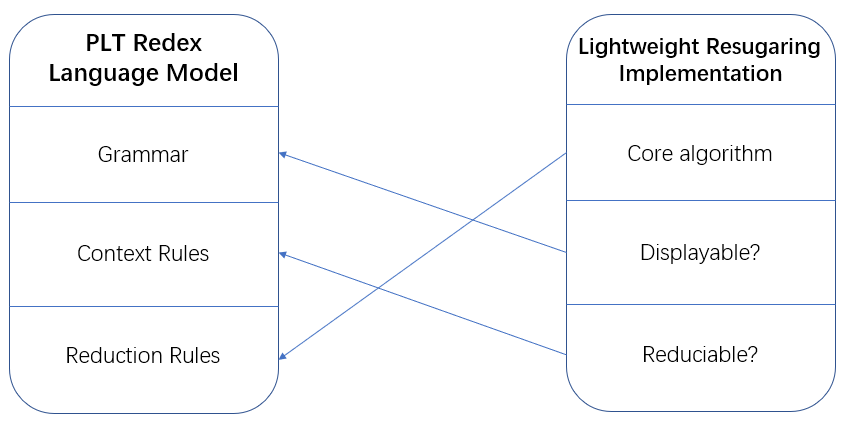
\includegraphics[width=12cm]{images/frame.png}
	\caption{framework of implementation}
	\label{fig:frame}
\end{figure}

The grammar of the whole language contains Coreexp, Surfexp and Commonexp as the language setting in sec\ref{sec3}. OtherSurfexp is of Surfexp and OtherCommonexp is of Commonexp. The identifier of any kind of expression is Headid of expression. If we need to add a syntactic sugar to the whole language, only three steps is needed.

\begin{enumerate}
\item Add grammar of the syntactic sugar.
\item Add context rules of the sugar, such that any sub-expressions can be reduced.
\item Add desugar rules of the sugar to reduction rules of the whole language.
\end{enumerate}

Then inputting an expression of the syntactic sugar to lightweight-resugaring will get the resugaring sequences.

\subsection{Evaluation}

We test some applications on the tool implemented using PLT Redex. Note that we set CBV's lambda calculus as terms in commonexp, because we need to output some intermediate sequences including lambda expressions in some examples. It's easy if we want to skip them.

\subsubsection{simple sugar}
\label{mark:simple}

We construct some simple syntactic sugar and try it on our tool. Some sugar is inspired by the first work of resugaring\cite{resugaring}. The result shows that our approach can process all sugar features of their first work.

We take a SKI combinator syntactic sugar as an example. We will show why our approach is lightweight.

\begin{flushleft}
	$S$ $\rightarrow$ $(\lambda _{N}~(x_{1}~x_{2}~x_{3})~(x_{1}~x_{2}~(x_{1}~x_{3})))$

	$K$ $\rightarrow$ $(\lambda _{N}~(x_{1}~x_{2})~x_{1})$

	$I$ $\rightarrow$ $(\lambda _{N}~(x)~x)$
\end{flushleft}

Although SKI combinator calculus is a reduced version of lambda calculus, we can construct combinators' sugar based on call-by-need lambda calculus in our CoreLang. For expression

 $(S~(K~(S~I))~K~xx~yy)$, we get the following resugaring sequences as following.
\begin{Codes}
    (S (K (S I)) K xx yy)
\CoreStep (((K (S I)) xx (K xx)) yy)
\CoreStep (((S I) (K xx)) yy)
\CoreStep (I yy ((K xx) yy))
\CoreStep (yy ((K xx) yy))
\CoreStep (yy xx)
\end{Codes}
% \begin{figure}[ht]
% 	\centering
% 	\parbox[t]{\textwidth}{
% 				\begin{center}
% 				{
% 					\small\selectfont
% 					(S (K (S I)) K xx yy)\\
% 					↓\\
% 					(((K (S I)) xx (K xx)) yy)\\
% 					↓\\
% 					(((S I) (K xx)) yy)\\
% 					↓\\
% 					(I yy ((K xx) yy))\\
% 					↓\\
% 					(yy ((K xx) yy))\\
% 					↓\\
% 					(yy xx)
% 				}
% 				\end{center}
% 			}
% 	\caption{SKI's resugaring sequences}
% 	\label{fig:SKI}
% \end{figure}

For existing approach, the sugar expression should firstly desugar to
\begin{flushleft}
$((\lambda _{N}
   (x_{1} x_{2} x_{3})
   (x_{1} x_{3} (x_{2} x_{3})))
  ((\lambda _{N} (x_{1} x_{2}) x_{1})
   ((\lambda _{N}
     (x_{1} x_{2} x_{3})
     (x_{1} x_{3} (x_{2} x_{3})))
    (\lambda _{N} (x) x)))
  (\lambda _{N} (x_{1} x_{2}) x_{1})
  xx
  yy)$
\end{flushleft}

Then in our CoreLang, the execution of expanded expression will contain 33 steps. For each step, there will be many attempts to match and substitute the syntactic sugars. We will omit more steps for a larger expression. So the unidirectional resugaring algorithm makes our approach lightweight.todo

\subsubsection{hygienic macro}
\label{mark:hygienic}

The second work\cite{hygienic} mainly processes hygienic macro compared to first work. We try a $Let$ sugar , which is a common hygienic sugar example, on our tool. Our algorithm can easily process hygienic macro without special data structure. The $Let$ sugar is define as follow

$(Let\;x\;v\;exp)$ $\rightarrow$ $(Apply\;(\lambda\;(x)\;exp)\;v)$

Take $(Let~x~1~(+~x~(Let~x~2~(+~x~1))))$ for an example. First, a temp expression

$(Apply\;(\lambda\;(x)\;(+~x~(Let~x~2~(+~x~1))))\;1)$

is needed. (case 5 or 6)Then one-step try on the temp expression, we will get

$(+~1~(Let~1~2~(+~1~1)))$ which is out of the whole language's grammar. In this case, it is not a good choice to desugar the outermost $Let$ sugar. Then we just apply the core-algo f on the sub-expression where the error occurs ($(+~x~(Let~x~2~(+~x~1)))$ in this example). So the right intermediate sequence $(Let~x~1~(+~x~3))$ will be get.

In practical application, we think resugaring for a unhygienic rewriting system is not interesting at all, because hygienic macro can be easily processed by rewriting system. So in the finally implementation of our tool, we just use PLT Redex's binding forms to deal with hygienic macros. But we did try it on the version without hygienic rewriting system.

\subsubsection{recursive sugar}
Recursive sugar is a kind of syntactic sugars where call itself or each other during the expanding. For example,

$(Odd\;e)$ $\rightarrow$ $(if\;(>\;e\;0)\;(Even\;(-\;e\;1)\;\#f))$

$(Even\;e)$ $\rightarrow$ $(if\;(>\;e\;0)\;(Odd\;(-\;e\;1)\;\#t))$

are typical recursive sugars. The previous works can process this kind of syntactic sugar easily, because boundary conditions are in the sugar itself.

Take $(Odd~2)$ as an example. The previous work will firstly desugar the expression using the rewriting system. Then the rewriting system will never start resugaring as Fig\ref{fig:odd} shows.

\begin{figure}[ht]
	\centering
	\parbox[t]{\textwidth}{
				\begin{center}
				{
					\small\selectfont
					(Odd 2)\\
					↓\\
					(if (> 2 0) (Even (- 2 1) \#f))\\
					↓\\
					(if (> (- 2 1) 0) (Odd (- (- 2 1) 1) \#t))\\
					↓\\
					(if (> (- (- 2 1) 1) 0) (Even (- (- (- 2 1) 1) 1) \#f))\\
					↓\\
					{\ldots}
				}
				\end{center}

			}
	\caption{Odd2's desugaring process}
\label{fig:odd}
\end{figure}

Then the advantage of our approach is embodied. Our lightweight approach doesn't require a whole expanding of sugar expression, which gives the framework chances to judge boundary conditions in sugars themselves, and showing more intermediate sequences. We get the resugaring sequences as Fig \ref{fig:rec} of the former example using our tool.

\begin{figure}[ht]
	\centering
	\parbox[t]{\textwidth}{
				\begin{center}
				{
					\small\selectfont
					(Odd 2)\\
					↓\\
					(Even (- 2 1))\\
					↓\\
					(Even 1)\\
					↓\\
					(Odd (- 1 1))\\
					↓\\
					(Odd 0)\\
					↓\\
					\#f
				}
				\end{center}

			}
	\caption{Odd2's resugaring sequences}
\label{fig:rec}
\end{figure}

We also construct some higher-order syntactic sugars and test them. The higher-order feature is important for constructing practical syntactic sugar. And for syntactic sugar's feature, it is of recursive sugar. Giving the following two higher-order syntactic sugar as examples.

\begin{flushleft}
	$(map\;e\;(list\;v_1\ldots))$→

	$(if\;(empty\;(list\;v_1\ldots))\;(list)\;(cons\;(e\;(first\;(list\;v_1\ldots)))\;(map\;e\;(rest\;(list\;v_1\ldots)))))$
\end{flushleft}

\begin{flushleft}
	$(filter\;e\;(list\;v_1\;v_2\ldots))$→

	$(if\;(e\;v_1)\;(cons\;v_1\;(filter\;e\;(list\;v_2\ldots)))\;(filter\;e\;(list\;v_2\ldots)))$

	$(filter\;e\;(list))$ → $(list)$
\end{flushleft}
These two syntactic sugars use different sugar forms to implement. For $Map$ sugar, we use if expression in CoreLang to constrain the boundary conditions. For $Filter$ sugar, we use two different parameters' form, which is another easy way for constructing syntactic sugar. The testing results show as Fig\ref{fig:map} \ref{fig:filter}.

\begin{figure}[ht]
	\centering
	\parbox[t]{\textwidth}{
				\begin{center}
				{
					\small\selectfont
					(map (λ (x) (+ 1 x)) (list 1 2 3))\\
					↓\\
					(cons 2 (map (λ (x) (+ 1 x)) (list 2 3)))\\
					↓\\
					(cons 2 (cons 3 (map (λ (x) (+ 1 x)) (list 3))))\\
					↓\\
					(cons 2 (cons 3 (cons 4 (map (λ (x) (+ 1 x)) (list)))))\\
					↓\\
					(cons 2 (cons 3 (cons 4 (list))))\\
					↓\\
					(cons 2 (cons 3 (list 4)))\\
					↓\\
					(cons 2 (list 3 4))\\
					↓\\
					(list 2 3 4)
				}
				\end{center}

			}
	\caption{Map's resugaring sequences}
\label{fig:map}
\end{figure}

\begin{figure}[ht]
	\centering
	\parbox[t]{\textwidth}{

				\begin{center}
				{
					\small\selectfont
					(filter (λ (x) (and (> x 3) (< x 6))) (list 1 2 3 4 5 6 7))\\
					↓\\
					(filter (λ (x) (and (> x 3) (< x 6))) (list 2 3 4 5 6 7))\\
					↓\\
					(filter (λ (x) (and (> x 3) (< x 6))) (list 3 4 5 6 7))\\
					↓\\
					(filter (λ (x) (and (> x 3) (< x 6))) (list 4 5 6 7))\\
					↓\\
					(cons 4 (filter (λ (x) (and (> x 3) (< x 6))) (list 5 6 7)))\\
					↓\\
					(cons 4 (cons 5 (filter (λ (x) (and (> x 3) (< x 6))) (list 6 7))))\\
					↓\\
					(cons 4 (cons 5 (filter (λ (x) (and (> x 3) (< x 6))) (list 7))))\\
					↓\\
					(cons 4 (cons 5 (filter (λ (x) (and (> x 3) (< x 6))) (list))))\\
					↓\\
					(cons 4 (cons 5 (list)))\\
					↓\\
					(cons 4 (list 5))\\
					↓\\
					(list 4 5)
				}

				\end{center}

			}
	\caption{Filter's resugaring sequences}
\label{fig:filter}
\end{figure}
\subsection{Compare to previous work}

As mentioned many times before, the biggest difference between previous resugaring approach and our approach, is that our approach doesn't need to desugar the sugar expresssion totally. Thus, our approach has the following advantages compared to previous work.

\begin{itemize}
	\item {\bfseries Lightweight} As the example at sec\ref{mark:simple}, the match and substitution process searchs all intermediate sequences many times. It will cause huge cost for a large program. So out approach---only expanding a syntactic sugar when necessarily, is a lightweight approach.
	\item {\bfseries Friendly to hygienic macro} Previous hygienic resugaring approach use a new data structure---abstract syntax DAG, to process resugaring of hygienic macros. Our approach simply finds hygienic error after expansion, and gets the correct reduction instead.
	\item {\bfseries More syntactic sugar features} The ability of processing recursive sugar is a superiority compared to previous work. The key point is that recursive syntactic sugar must handle boundary conditions. Our approach handle them easily by not necessarily desugaring all syntactic sugars. Higher-order functions, as an important feature of functional programming, was supported by many daily programming languages. So the ability on higher-order sugar is important.
	\item {\bfseries Rewriting rules based on reduction semantics} Any syntactic sugar that can expressed by reduction semantics can be used in our approach. It will give more possible forms for constructing syntactic sugars. todo:example?
\end{itemize}

%!TEX root = ./main.tex
\section{The Mixed Language for Resugaring}
\label{sec:language}

Different from the existing approach that clearly separates the surface language (defined by syntactic sugars over the core language) from the core languages, we intentionally combine them as one mixed language, allowing free use of the language constructs in both languages. In this section, we will introduce our mixed language, which is the basic of our approach.

Note that this section discusses the second step in Section \ref{sec2}, while
assuming that the first step of calculating the context rules for the surface language has been done. The first step will be discussed later in Section \ref{sec:algo}.

%Note that the mixture is unfinished until the process in next section, because of the lack of context rules for expressions headed with \m{SurfHead}.
%We assume that the evaluation of the core language is  compositional (as the definition in \cite{hygienic}), that is, for evaluation contexts $C_1$ and $C_2$, $C_1[C_2]$ is also an evaluation context.

\begin{figure}[t]
	\begin{flushleft}
	{\footnotesize
	\[
	\begin{array}{lllll}
	\m{CoreExp} &::=& x  & \note{variable}\\
	&~|~& v  & \note{value}\\
	&~|~& (\m{CoreHead}~\m{CoreExp}_1~\ldots~\m{CoreExp}_n) & \note{constructor}\\
	\\
	\m{SurfExp} &::=& x  & \note{variable}\\
	&~|~& v  & \note{value}\\
	&~|~& (\m{SurfHead}~\m{SurfExp}_1~\ldots~\m{SurfExp}_n) & \note{sugar constructor}\\
	\end{array}
	\]
	}
	\end{flushleft}


		\caption{Core and Surface Expressions}
		\label{fig:expression}
	\end{figure}

\subsection{Core Language}

Any language can serve as our core language. For simplicity, we assume that the form of the expressions in our core language is defined as in Fig. \ref{fig:expression}. An expression can be a variable, a value, or a (language) constructor expression. Here, $\m{CoreHead}$ stands for a language constructor such as $\m{if}$ and $\m{let}$. Also, the sub-expressions can be nested for supporting expressions like \Code{(let (x e) $\ldots$)}. To be concrete, in this paper we will use the core language defined in Fig.  \ref{fig:core} to demonstrate our approach. It is a usual functional language and its semantics is defined by the context rules and the reduction rules. Here the [e/x] denotes capture-avoiding substitution.

\begin{figure*}[t]
\begin{subfigure}{0.55\linewidth}
\[
{\footnotesize
		\begin{array}{lcl}
		\m{CoreExp} &::=& \Code{(CoreExp~CoreExp~...)} ~~\note{// application}\\\\

		&|& \m{(if~CoreExp~CoreExp~CoreExp)} ~~\note{// condition}\\
		&|& \m{(let~(x~CoreExp)~CoreExp)} ~~\note{// binding}\\
		&|& \m{(listop~CoreExp)} ~~\note{// first, rest, empty?}\\
		&|& \m{(cons~CoreExp~CoreExp)} ~~\note{// data structure of list}\\
		&|& \m{(arithop~CoreExp~CoreExp)} ~~\note{// +, -, *, /, >, <, =}\\
		&|& \m{x} ~~\note{// variable}\\
		&|& \m{value}\\
		\m{value} &::=& \m{($\lambda$~(x~...)~CoreExp)} ~~\note{// call-by-value}\\
		&|& \m{c} ~~\note{// boolean, number and list}
		\end{array}
}
\]
\caption{Syntax}
\end{subfigure}
\begin{subfigure}{0.4\linewidth}
\[
{\footnotesize
		\begin{array}{lcl}
		\Code{C} &::=& \Code{(value~...~C~CoreExp~...)}\\
		&|& \Code{(if~C~CoreExp~CoreExp)}\\
		&|& \Code{(let~(x~C)~CoreExp)}\\
		&|& \Code{(listop~C)}\\
		&|& \Code{(cons~C~CoreExp)}\\
		&|& \Code{(cons~value~C)}\\
		&|& \Code{(arithop~C~CoreExp)}\\
		&|& \Code{(arithop~value~C)}\\
		&|& [\bigcdot]\\[1.5em]
		\end{array}
}
\]
\caption{Context Rules}
\end{subfigure}

\begin{subfigure}{0.99\linewidth}
	\[
{\footnotesize
		\begin{array}{lcl}
		\Code{(($\lambda$~($x_1$~$x_2$~...)~CoreExp)~$\m{value}_1$~$\m{value}_2$~...)} &\redc{}{}& \Code{(($\lambda$~($x_2$~...)~CoreExp[$\m{value}_1$/$x_1$])~$\m{value}_2$~...)}\\

		\Code{(if~$\m{\true}$~$\m{CoreExp}_1$~$\m{CoreExp}_2$)}&\redc{}{}& \Code{$\m{CoreExp}_1$}\\
		\Code{(if~$\m{\false}$~$\m{CoreExp}_1$~$\m{CoreExp}_2$)}&\redc{}{}& \Code{$\m{CoreExp}_2$}\\
		\Code{(let~($x$~$\m{value}$)~CoreExp)}&\redc{}{}&\Code{CoreExp[\m{value}/$x$]}\\
		\ldots&&
		\end{array}
}
\]
	\caption{Part of Reduction Rules}
\end{subfigure}

\caption{A Core Language}
\label{fig:core}
\end{figure*}

The evaluator of our core language is driven by evaluation rules (context rules and reduction rules), with two natural assumptions. First, the evaluation is deterministic, in the sense that any expression in the core language will be reduced by a unique reduction sequence (defined by the context rules). Second, the context rules have no side conditions, which excludes the following rules (here $f_1$, $f_2$ are two auxiliary functions).

{\footnotesize
\[
\begin{array}{lll}
\m{C}& ::= & (\m{notif}~[\bigcdot]~e_2~e_3)\\
&|& (\m{notif}~v_1~[\bigcdot]~e_3), \qquad \m{when}~(f_1~v_1)\\
&|& (\m{notif}~v_1~e_2~[\bigcdot]), \qquad \m{when}~(f_2~v_1)
\end{array}
\]}


\subsection{Surface Language}
\label{mark:suflang}

A surface language is defined by a set of syntactic sugars, together with some elements in the core language, such as values and variables. The expression of a surface language has a similar form with that of the core as shown in Fig.  \ref{fig:expression}. To separate surface language's \m{Head} from that of the core language, we capitalize the first letter of surface language's \m{Head}.


A syntactic sugar \m{SurfHead} is defined by a desugaring rule in the following form
\[
\drule{(\m{SurfHead}~e_1~e_2~\ldots~e_n)}{\m{exp}} %\todo{\text{font size in drule}}
\]
where its left-hand side (LHS) is a pattern and its right-hand side (RHS) is an expression of the mixed language (described in the next section).
%The LHS may be nested, so we can write sugars like \Code{(SurfHead ($e_1$ ($e_2$ $e_3$)) $\ldots$ $e_n$)}.
For instance, we may define syntactic sugar \m{And} by
\[
\drule{(\m{And}~e_1~e_2)}{(\m{if}~e_1~e_2~\m{\false})}.
\]

In the following, we give some interesting cases for defining sugars, showing our extension and demonstrating its power in defining surface language.

\subsubsection{Sugars with no Arguments}
A sugar definition does not need to have pattern variables at LHS, because we can use the $\lambda$ abstraction in the core language. For example, we can define the sugar of SKI combinator by following rules. ($\lambda_N$ here is the call-by-need lambda calculus.)
\[
\begin{array}{l}
\drule{\m{S}}{\Code{($\lambda_N$ ($\m{x}_1$ $\m{x}_2$ $\m{x}_3$) ($\m{x}_1$ $\m{x}_2$ ($\m{x}_1$ $\m{x}_3$)))}}\\
\drule{\m{K}}{\Code{($\lambda_N$ ($\m{x}_1$ $\m{x}_2$) $\m{x}_1$)}}\\
\drule{\m{I}}{\Code{($\lambda_N$ (x) x)}}
\end{array}
\]

\subsubsection{Sugars with Linear Use of Pattern Variables}
We assume that any pattern variable (e.g., $e_1$) in LHS appears only once in RHS for the syntactic sugar.
If we need to use a pattern variable multiple times in RHS, a \m{let} binding may be used.\footnote{Of course, we can add the support for multiple appearance for a pattern variable by some special judgements. But we just make it simple for presentation.} To see the problem of multiple uses of a variable, suppose we define a sugar by
$
\drule{(\m{Twice}~e_1)}{(+~e_1~e_1)}.
$
If we execute \Code{(Twice (+ 1 1))}, it will first be desugared to \Code{(+ (+ 1 1) (+ 1 1))}, then reduced to \Code{(+ 2 (+ 1 1))} by one step. The sub-expression \Code{(+ 1 1)} has been reduced but should not be resugared to the surface, because the other \Code{(+ 1 1)} has not been reduced yet.
In this paper, we just use a \m{let} binding to resolve this problem, and define it as
\[
\drule{(\m{Twice}~e_1)}{\Code{(let (x $e_1$) (+ x x))} }.
\]

\subsubsection{Hygienic Sugars}
The use of \m{let} binding is useful, but it introduces the hygienic problem for desugaring. For example, considering we have the following syntactic sugar
\[
\drule{\Code{(HygienicAdd $e_1$ $e_2$)}}{\Code{(let (x $e_1$) (+ x $e_2$))}}
\]
for the program \Code{(let (x 2) (HygienicAdd 1 x))}, it would be desugared by a simple expansion to the unexpected expression \Code{(let (x 2) (let x 1 (+ x x)))}. We will show how we solve this problem later.

\subsubsection{Recursive and Higher Order Sugars}
In the desugaring rule, we relax the ordinary restriction that RHS must be a $\m{CoreExp}$. This makes it possible to define recursive sugars as follows:

\[\begin{array}{l}
	\drule{\Code{(Filter $e$ (list $v_1$ $v_2$ ...))}}{}\\
	\quad
	\Code{ (let (f $e$) (if (f $v_1$)}\\
	\qquad\qquad\qquad\qquad\ \Code{ (cons $v_1$ (Filter f (list $v_2$ ...)))}\\
	\qquad\qquad\qquad\qquad\ \Code{ (Filter f (list $v_2$ ...))))}\\
\\
	\drule{\Code{(Filter $e$ (list))}}{\Code{(list)}}
	\end{array}
\]

Moreover, we allow more involved recursive syntactic sugars, which is ill-formed from the traditional view of desugaring. For example, the following sugar is not allowed by simple desugaring \cite{resugaring}, because the expansion of sugar will not stop. Fortunately, it is allowed in our context.
\[
\begin{array}{l}
\drule{(\m{Odd}~e)}{(\m{let}~(x~e)~(\m{if}~(>~x~0)~(\m{Even}~(-~x~1))~\m{\false}))}\\
\drule{(\m{Even}~e)}{(\m{let}~(x~e)~(\m{if}~(>~x~0)~(\m{Odd}~(-~x~1))~\m{\true}))}
\end{array}
\]
%However, the "semantics" of such syntactic sugar is sound, so we have a chance to handle this case by our lazy desugaring. This can be practical, though we should have written the \m{Odd, Even} sugars by a pattern matching like \m{Filter}.
%Sometimes we can only use an inline condition like \Code{(empty? x)} to judge the branch as the following \m{Map} sugar.

As another example, we can define the \m{Map} sugar as follows.
\[
\begin{array}{l}
\drule{\Code{(Map $e_1$ $e_2$)}}{}\\
\quad\Code{(let (f $e_1$)}\\
\qquad\Code{(let (x $e_2$)}\\
\qquad\quad

\Code{(if (empty? x)}\\
\qquad\qquad\quad\Code{(list)}\\
\qquad\qquad\quad\Code{(cons (f (first x)) (Map f (rest x))))))}
\end{array}
\]
In this case, our approach can handle something which is hard to deal with by traditional desugaring.

\medskip
We will return to the examples in this section to show how resugaring can be done for the  sugars that are defined here.



\subsection{Mixed Language}
\begin{figure}[t]
\begin{centering}
{\footnotesize
\[
			\begin{array}{lcl}
			\m{Exp} &::=& \m{DisplayableExp}\\
			&|& \m{MixedExp}\\
			\\
			\m{DisplayableExp} &::=& \m{(SurfHead~DisplayableExp~$\ldots$)}\\
			&|& \m{(CommonHead~DisplayableExp~$\ldots$)}\\
			&|& v\\
			&|& x\\
			\\
			\m{MixedExp} &::=& \m{(SurfHead~MixedExp~$\ldots$)}\\
			&|& \m{(CoreHead~MixedExp~$\ldots$)}\\
			&|& v\\
			&|& x\\
			\end{array}
			\]
}

\end{centering}
\caption{Syntax of the Mixed Language\todo{explain}}
\label{fig:mix}
\end{figure}

A mixed language for resugaring combines the surface language and the core language, with the mixture of syntax, context rules, and reduction rules. As discussed at the beginning of this section, since  the context rules of the sugars are calculated by the algorithm later, we assume here that we have their context rules.

\subsubsection{Mixing Syntax}
The mixed syntax is described in Fig.  \ref{fig:mix}.
%
The differences between expressions in our core language and those in our surface language are identified by their \m{Head}. But there may be some expressions in the core language which are also used in the surface language for convenience, or to say, we need some core language's expressions to help us get better resugaring sequences. So we take \m{CommonHead} as a subset of the \m{CoreHead}, which can be displayed in resugaring sequences (just as the \m{CommonExp} in our Section \ref{sec2}). Then if any sub-expression in an expression contains no \m{CoreHead} except for \m{CommonHead}, we should let them displayed during the evaluation process (named \m{DisplayableExp}). Otherwise, the expression should not be displayed. We just use a \m{MixedExp} expression to represent the expressions that are unnecessarily displayed for concision, and discuss more on \m{DisplayableExp}  in Section \ref{mark:correctness}.





As an example, for the core language in Fig.  \ref{fig:core},
we may assume \m{arithop}, \m{$\lambda$} (call-by-value lambda calculus), \m{cons} as \m{CommonHead}, \m{if}, \m{let}, \m{listop} as \m{CoreHead} but out of \m{CommonHead}. This will allow \m{arithop}, \m{$\lambda$} and \m{cons} to appear in the resugaring sequences, and thus display more useful intermediate steps during resugaring.

\begin{figure}[t]
	\centering
	\begin{subfigure}{0.3\linewidth}{\footnotesize
		\begin{flushleft}
			\[
			\begin{array}{lcl}
			\m{C} &:=& (\m{CoreHead1}~$\ldots$~C~$\ldots$)\\
			&|& (\m{CoreHead2}~$\ldots$~C~$\ldots$)\\
			&|& $\ldots$\\
			&|&[\bigcdot]\\[4em]
			\end{array}
			\]
			\end{flushleft}
		\caption{Core's Context Rules}
		\label{fig:corecontext}
	}
	\end{subfigure}
	\begin{subfigure}{0.3\linewidth}{\footnotesize
		\begin{flushleft}
			\[
			\begin{array}{lcl}
			\m{C} &:=& (\m{SurfHead1}~$\ldots$~C~$\ldots$)\\
			&|& (\m{SurfHead2}~$\ldots$~C~$\ldots$)\\
			&|& $\ldots$\\
			&|&[\bigcdot]\\[4em]
			\end{array}
			\]
			\end{flushleft}
		\caption{Surface's Context Rules}
		\label{fig:surfcontext}
	}
	\end{subfigure}
	\begin{subfigure}{0.3\linewidth}{\footnotesize
		\begin{flushleft}
			\[
			\begin{array}{lcl}
			\m{C} &:=& (\m{CoreHead1}~$\ldots$~C~$\ldots$)\\
			&|& (\m{CoreHead2}~$\ldots$~C~$\ldots$)\\
			&|& $\ldots$\\
			&|& (\m{SurfHead1}~$\ldots$~C~$\ldots$)\\
			&|& (\m{SurfHead2}~$\ldots$~C~$\ldots$)\\
			&|& $\ldots$\\
			&|&[\bigcdot]\\
			\end{array}
			\]
			\end{flushleft}
		\caption{Mixed's Context Rules}
		\label{fig:mixedcontext}
	}
	\end{subfigure}

\caption{Mixture of Context Rules}
\label{fig:mixofcontext}
\end{figure}

\subsubsection{Mixing Context and Reduction Rules}

The context rules specify the computational order for an expression based on the \m{Head}, so that they can be simply mixed as described in Fig. \ref{fig:mixofcontext}. And if we want to limit the unique reduction of an expression, we should modify the desugaring rules to be correct for the reduction. For example, if we have the context rules as in Fig. \ref{fig:mixcontext}, then for the expression
\[
	\Code{(if (And (And \true~\true) \false) \false~\true)}
\]
it will reduce at the sub-expression \Code{(And (And \true~\true) \false)}. But the outer \m{And} sugar should not be expanded according to the context rules of \m{And}, so we should change
\[
	\drule{(\m{And}~e_1~e_2)}{(\m{if}~e_1~e_2~\m{\false})}
\]
to
\[
	\drule{(\m{And}~v_1~e_2)}{(\m{if}~v_1~e_2~\m{\false})}.
\]
\hmodify{Question}{What is $v$? This example is a bit difficult to understand.}

After the mixture of reduction rules in the core language ($\redc{}{}$) and the  desugaring rules for the syntactic sugars in the surface language ($\drule{}{}$), any expression in the mixed language can be reduced step by step. For example, in the mixed language, some expressions with \m{CoreHead} may contain sub-expressions with \m{SurfHead}. We process these expressions by the context rules of the core language, so that the reduction rules of the core language and the desugaring rules of surface language can be mixed as a whole
 (the $\redm{}{}$ in Fig. \ref{fig:mixexample}). For example, suppose we have the context rule of \m{if} expression\footnote{Another presentation of \Code{(if $[\bigcdot]$ e e)}. Use this here for convenience.}
\[
\infer{(\m{if}~e_1~e_2~e_3) \rightarrow (\m{if}~e_1'~e_2~e_3)}{e_1 \rightarrow e_1'}
\]
then if $e_1$ is headed with \m{CoreHead}, the reduction will use the \m{CoreHead}'s reduction rules recursively. So does it if $e_1$ headed with \m{SurfHead}. Finally, the $e_1$ is reduced to a value, then we can use the reduction rule of \m{if}.

%!TEX root = ./main.tex
\section{Implementation}
\label{sec4}


We have implemented our resugaring approach using PLT Redex \cite{SEwPR}, a semantic engineering tool based on reduction semantics \cite{reduction}. We show several case studies to demonstrate the power of our approach. Some examples discussed in this section are in Fig. \ref{fig:resugaring}. Note that we set call-by-value lambda calculus as terms in \m{CommonExp}, because we want to output some intermediate expressions including lambda calculus in some examples. It is easy if we want to skip them.

\begin{figure}[t]
	\centering
	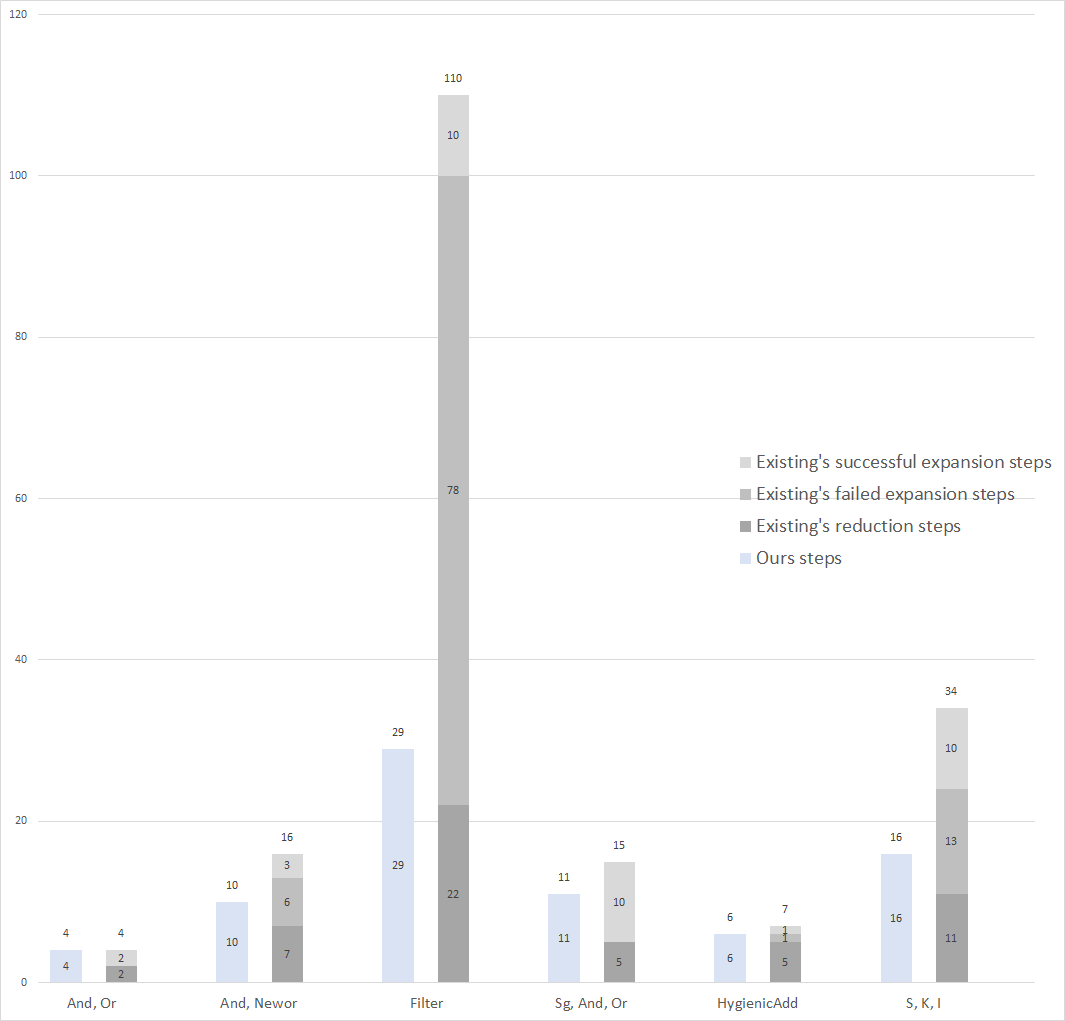
\includegraphics[width=0.471\textwidth]{images/efficiency.png}
	\caption{Comparison on Reduction Steps}
	\label{fig:step}
\end{figure}

To show the efficiency of our approach, we use the number of reduction steps comparing to the existing approach as the metrics. Figure \ref{fig:step} shows the difference between the two approaches. Notice that both approaches have pre-processing---for the existing one, it is to desugar the programs to the core language together with some tags; for ours, it is to calculate the context rules of syntactic sugars. We do not consider the steps during pre-processing. Besides, we derive the reduction steps of the existing approach into three different kinds---the reductions in the core language, the reverse expansion with failed resugaring, the reverse expansion with successful resugaring.  Use the following example to see the difference. Consider a sugar named \m{Hard} with two arguments, which has many reduction steps after desugared. Assuming for specific $e_1$ and $e_2$, the \Code{(Hard $e_1$ $e_2$)} after fully desugared has 100 reduction steps (e.g. finally to \#f), and only 1 intermediate step ($\m{step}_n$) can be resugared (e.g. to \Code{(Hard $v_1$ $e_2$)}). Then for \Code{(And (Hard $e_1$ $e_2$) \#t)}, although all the 100 steps in the core language try the reverse desugaring, only \Code{(if $\m{step}_n$ \#t \#f)} (2 steps on \m{And}, \m{Hard}) and \Code{(if \#f \#t \#f)} (1 step on \m{And}) are successful. Other 98 attempts will be failed with 98 failed reverse expansion steps on \m{And}.

\[
{\footnotesize
	\begin{array}{lcl}
	\text{Surface}&&\text{Core}\\
	\Code{(And (Hard $e_1$ $e_2$) \#t)}&\xrightarrow{desugar}&\Code{(if $\m{step}_0$ \#t \#f)}\\
	\qquad\quad\dashdownarrow& &\qquad\qquad\downarrow\\
	\Code{(And $\m{step}_1$ \#t)}&\xleftarrow{resugar}&\Code{(if $\m{step}_1$ \#t \#f)}\\
	\qquad\quad\vdots& &\qquad\qquad\vdots\\
	\Code{(And (Hard $v_1$ $e_2$) \#t)}&\xleftarrow{resugar}&\Code{(if $\m{step}_n$ \#t \#f)}\\
	\qquad\quad\vdots& &\qquad\qquad\vdots\\
	\Code{(And \#f \#t)}&\xleftarrow{resugar}& \Code{(if \#f \#t \#f)}\\
	\qquad\quad\dashdownarrow& &\qquad\qquad\downarrow\\
	\Code{\#f}&& \Code{\#f}\\
\end{array}
}
\]


The general tendency is---the more complex the sugar is, the more steps will our approach save. Note that if the RHS of a syntactic sugar is huge, one-step reduction of the reverse desugaring will also be complex, because huge sugars will contain many failed attempts to resugar. So avoiding reverse expansion of syntactic sugar can improve the efficiency for practical use because programs are usually not that small like the demos.

%!TEX root = ./main.tex
\section{Extensions}
\label{sec5}
\ycomment{}
\subsection{Model Assumption and A Black-Box Extension}


As we mentioned in the introduction (Section \ref{mark:mention}), our approach assumes a more specific model (evaluation rules) compared to the existing approach (black-box stepper). Here is a small gap between the motivation of the existing approach and ours---the existing approach focused mainly on a tool for existing language, while our approach considered more on a meta-level feature for language implementation. Some examples in next chapter will show how the lazy desugaring solves some problems in practice.

In addition, as what we need for the lazy desugaring is just the computational order of the syntactic sugar, we can make an extension for the resugaring algorithm to work with only a black-box core language stepper. The most important difference between the black-box stepper and the evaluation rules is the computational order---while the same language behaves uniquely, the evaluation rules can show the computational order statically (without running the program). So when meeting the black-box stepper for the core language, we can just use some simple program to "get" the computational order of the core language as the following example  shows: we simply let the sub-expressions of a \m{Head} be some reducible expressions and test the computational order.

\begin{center}\footnotesize
	\Code{(if $\m{tmpe}_1$ $\m{tmpe}_2$ $\m{tmpe}_3$)}\\ $\Downarrow_{stepper}$\\ \Code{\qquad\qquad\qquad\qquad\;\;(if $\m{tmpe}_1$' $\m{tmpe}_2$ $\m{tmpe}_3$)}\note{//getting a context rule}\\ $\Downarrow_{getnext}$\\ \Code{(if $\m{tmpv}_1$ $\m{tmpe}_2$ $\m{tmpe}_3$)}\\ $\Downarrow_{stepper}$\\ \qquad\Code{$\m{tmpe}_i$}\note{//no more rules}\\
\end{center}


But that's not enough---the core language and the surface language cannot be mixed easily because of the lack of evaluation rules for the core language. We should do the same try during the evaluation to make the core language's stepper useful when meeting some surface language's expression. Here we give a dynamic on-step reduction of the mixed language. Note that here we only define the reduction for unnested syntactic sugar for convenience. It is easy to extend to nested sugar (but so huge to express). 

\begin{Def}[Dynamic mixed language's one-step reduction $\redm{}{}$] Defined in Fig.  \ref{fig:dynamic}.
\end{Def}
\begin{figure*}[t]\footnotesize
\infrule[CoreRed]
{ \forall~i.~e_i\in \m{CoreExp}\\
\redc{(\m{CoreHead}~e_1~\ldots~e_n)}{e'}}
{\redm{(\m{CoreHead}~e_1~\ldots~e_n)}{e'}}
\infrule[CoreExt1]
{ \forall~i.~tmp_i= (e_i \in \m{SurfExp}~?~\m{tmpe}~:~e_i)\\
\redc{(\m{CoreHead}~tmp_1~\ldots~tmp_i~\ldots~tmp_n)}{(\m{CoreHead}~tmp_1~\ldots~tmp_i'~\ldots~tmp_n)}}
{\redm{(\m{CoreHead}~e_1~\ldots~e_i~\ldots~e_n)}{(\m{CoreHead}~e_1~\ldots~e_i'~\ldots~e_n)}\\where~\redm{e_i}{e_i'}}
\infrule[CoreExt2]
{ \forall~i.~tmp_i= (e_i \in \m{SurfExp}~?~\m{tmpe}~:~e_i)\\
\redc{(\m{CoreHead}~tmp_1~\ldots~tmp_n)}{e'}~\note{// not reduced in sub-expressions}}
{\redm{(\m{CoreHead}~e_1~\ldots~e_n)}{e'[e_1/tmp_1~\ldots~e_n/tmp_n]}}
\infrule[SurfRed1]
{\drule{(\m{SurfHead}~x_1~\ldots~x_i~\ldots~x_n)}{e}~\\
\exists i.\, \redm{e[e_1/x,\ldots,e_i/x_i,\ldots,e_n/x_n]}{e[e_1/x,\ldots,e_i'/x_i,\ldots,e_n/x_n]}~\&~
\redm{e_i}{e_i''}
}
{\redm{(\m{SurfHead}~e_1~\ldots~e_i~\ldots~e_n)}{(\m{SurfHead}~e_1~\ldots~e_i''~\ldots~e_n)}}
\infrule[SurfRed2]
{\drule{(\m{SurfHead}~x_1~\ldots~x_i~\ldots~x_n)}{e}\\
\not \exists i.\, \redm{e[e_1/x_1,\ldots,e_i/x_i,\ldots,e_n/x_n]}{e[e_1/x_1,\ldots,e_i'/x_i,\ldots,e_n/x_n]~\&~
\redm{e_i}{e_i''}}
}
{\redm{(\m{SurfHead}~e_1~\ldots~e_i~\ldots~e_n)}{e[e_1/x_1,\ldots,e_i/x_i,\ldots,e_n/x_n]}}
\footnotesize{where~\m{tmpe}~is~any~reduciable~\m{CoreExp}~expression}
\caption{Dynamic Reduction}
\label{fig:dynamic}
\end{figure*}

Putting them in words. For expression \Code{(SurfHead $e_1$ $\ldots$ $e_n$)}, as we discussed in Section \ref{mark:correct}, only reduction on the $e_i$ of the sugar's $LHS$ will not destroy the $RHS$'s form. So we can just take a try after the expansion of \m{SurfHead}. 

For an expression \Code{(CoreHead $e_1$ $\ldots$ $e_n$)}  whose sub-expressions contain \m{SurfExp}, replacing all \m{SurfExp} sub-expressions with any reducible core language's expression $\m{tmpe}_i$ . Then getting a result after inputting the new expression $e'$ to the original black-box stepper. Then two possible cases come.

If reduction appears at a sub-expression at $\m{tmpe}_i$'s location, then the stepper with the extension should return \Code{(CoreHead $e_1$ $\ldots$ $e_i'$ $\ldots$ $e_n$)}, where $e_i'$ is $e_i$ after the mixed language's one-step reduction ($\redm{}{}$) as the following example (rule $\mathtt{CoreExt1}$)
\begin{center}\scriptsize
	\Code{(if (and e1 e2) (or e1 e2) \#f)}\\ $\Downarrow_{replace}$\\ \Code{(if (not \#t) (not \#t) \#f)}\\ $\;\;\Downarrow_{blackbox}$\\ \Code{(if \#f (not \#t) \#f)}\\ $\quad\Downarrow_{reduction}$\\ \Code{(if (if e1 e2 \#f) (or e1 e2) \#f)}
\end{center}

Otherwise (no reduction on $\m{tmp}_i$), the stepper should return \Code{$e'$}, with all the replaced sub-expressions replacing back (rule $\mathtt{CoreExt2}$).
\begin{center}\scriptsize
	\Code{(if \#t (and ...) (or ...))}\\ $\Downarrow_{replace}$ \\\Code{ (if \#t $\m{tmpe}_2$ $\m{tmpe}_3$)}\\ $\;\;\Downarrow_{blackbox}$\\  \Code{$\m{tmpe}_2$}\\ $\quad\;\;\;\Downarrow_{replaceback}$\\ \Code{(and ...)}
\end{center}
We call the extension "one-step-try", because it tries one step on the expression in the black-box stepper. The extension will not violate the properties of the original core language's evaluator. It is obvious that the evaluator with the extension will reduce at the sub-expression as it needs in the core language, if the reduction appears in a sub-expression. The stepper with extension behaves the same as mixing the evaluation rules of the core language and desugaring rules of surface language.

But something goes wrong when substitution takes place during \m{CoreExt2}. For a program like \Code{(let (x 2) (Sugar x y))} as an example, it should reduce to \Code{(Sugar 2 y)} by the \m{CoreRed2} rule, but got \Code{(Sugar x y)} by the \m{CoreExt2} rule. So when using the extension of black-box stepper's rule (\m{ExtRed2}), we need some other information about in which sub-expression a substitution will occur. Then for these sub-expressions, we need to do the same substitution before replacing back. The substitution can be got by a similar idea as the dynamic reduction in our simple core language's setting. For example, we know the third sub-expression of an expression headed with \m{let} is to be substituted. we should first try \Code{(let (x 2) x)}, \Code{(let (x 2) y)} in one-step reduction to get the substitution [2/x], then, getting \Code{(Sugar 2 y)}.

Then for any sugar expression, we can process them dynamically by "one-step-try" like the example in Fig.  \ref{example:try}. (The bold \m{Head} means trying on this expression.)
\example{
\[
{\footnotesize
	\begin{array}{lcl}
	\text{resugaring}&&\text{one-step-try}\\
	\Code{({\bfseries And} (Or \#t \#f)}&\xrightarrow{try}&\Code{(if ({\bfseries Or} \#t \#f)}\\
	\Code{\qquad\hspace{0.5em}(And \#f \#t))}&&\Code{\qquad(And \#f \#t)}\\
	& &\Code{\qquad\#f)}\\
	\qquad\quad\dashdownarrow& &\qquad\qquad\downarrow\\
	\Code{(And ({\bfseries Or} \#t \#f)}& &\Code{(And ({\bfseries if} \#t \#t \#f)}\\
	\Code{\qquad\hspace{0.5em}(And \#f \#t))}&&\Code{\qquad\hspace{0.5em}(And \#f \#t))}\\
	\qquad\quad\dashdownarrow& &\qquad\qquad\downarrow\\
	\Code{({\bfseries And} \#t}&\xrightarrow{try}&\Code{({\bfseries if} \#t}\\
	\Code{\qquad\hspace{0.5em}(And \#f \#t))}&&\Code{\qquad\hspace{0.5em}(And \#f \#t)}\\
	& &\Code{\qquad\hspace{0.5em}\#f)}\\
	\qquad\quad\dashdownarrow& &\qquad\qquad\downarrow\\
	\Code{({\bfseries And} \#f \#t)}&\xrightarrow{try}&\Code{({\bfseries if} \#f \#t \#f)}\\
	\qquad\quad\dashdownarrow& &\\
	\Code{\#f}& &\\
\end{array}
}
\]
}{Example of One-Step-Try}{example:try}

\subsection{\ycomment{Side effect}}


Side effect is a special issue in resugaring. In the previous section, we described the core language as a pure functional language, but some side effects are allowed according to the algorithm. Because the computational order calculated is correct, side effects does not matter if we only consider the evaluation result. But the actual issue is the output of resugaring sequences. Assuming that the core language can process side effects by adding an environment, with a \m{set} expression changing a value of a variable and a \m{begin} expression evaluating all sub-expressions and returning the last result in the core language for using the environment.

If \Code{(begin e ...)} has the context rules
\[
	{\footnotesize
	\begin{array}{lcl}
		\Code{C}&:==&\Code{(\m{begin~C})}\\
		& | &\Code{(\m{begin~C~e~$\ldots$})}\\
		& | &[\bigcdot]
	\end{array}
	}
\]
and reduction rules
\[
{\footnotesize
		\begin{array}{lcl}
		\Code{(begin~$\m{v}_1$~$\m{e}_2$~...)} &\redc{}{}& \Code{(begin~$\m{e}_2$~...)}\\
		\Code{(begin~v)} &\redc{}{}& \Code{v}\\
		\end{array}
}
\]
given a syntactic sugar 
\[\drule{\Code{(inc x y)}}{\Code{(begin (set x (+ x y)) x)}}\]
and for the following expression \Code{(let (x 1) (inc (+ 2 1) x))}, we will have the following evaluation sequence in the core language (omitted the desugaring process).
\begin{center}
	\Code{(let (x 1) (begin (set x (+ (+ 2 1) x) x)))}\\
	$\downarrow$\\
	\Code{(begin (set x (+ (+ 2 1) x) x)) [x:1]}\\
	$\downarrow$\\
	\Code{(begin (set x (+ 3 x) x)) [x:1]} {\footnotesize (inc (+ 2 1) x)}\\

\end{center}
\todo{}



\subsection{Possible Extensions}

So far, our desugaring rules are of a simple form. What if we need a more complex form to describe more complex semantics for syntactic sugar? For example, we may need a type system for checking during desugaring; we may specify the binding of syntactic sugar for more general hygiene; we may use some other functions to help the desugaring. All of these extensions are possible as long as the following conditions are satisfied.
\begin{enumerate}
	\item \emph{Compositional}: Generally speaking, the desugaring order and should not affect the semantics of a sugar expression. Otherwise, the lazy desugaring will not be correct.
	\item \emph{Unique Computational Order}: For any rules of syntactic sugar, the context rules should limit an expression to have only one computational order. Otherwise, the algorithm \m{calcontext} will not be deterministic.
	\item \emph{Clear Semantic}: If a syntactic sugar's desugaring rule is ambiguous or wrong, the algorithm \m{calcontext} may go wrong.
\end{enumerate}

For instance, we may need a desugaring rule like
\[
\drule{\Code{(Sugar $e_1$ $e_2$ $\ldots$ $e_n$)}}{\Code{(if (Helper $e_1$ $e_2$) $\ldots$)}}
\]
where \m{Helper} is an external function, that means we don't have the evaluation rules of \m{Helper}. In this case, we have to force the expansion of sugar expressions headed by \m{Sugar}. We describe how to force the desugaring in Section \ref{mark:simple}.





%!TEX root = ./main.tex
\section{Related Work}
\label{sec6}
%Explain the work that are related to your problem, and to your three contributions.
\todo{checking the sentense}

As discussed many times before, our work is much related to the pioneering work of \emph{resugaring} in \cite{resugaring}. The idea of "tagging" and "reverse desugaring" is a clear explanation of "resugaring", but it becomes very complex when the RHS of the desugaring rule becomes complex. Our approach does not need to reverse desugaring and is more powerful, and efficient.
For hygienic resugaring, compared with the approach of using DAG to solve the variable binding problem in \cite{hygienic}, our approach of "lazy desugaring" can achieve a kind of natural hygiene within our core language.



\emph{Macros as multi-stage computations} \cite{multistage} is a work related to our lazy expansion for sugars. Some other researches \cite{modularstaging} about multi-stage programming \cite{MSP} indicate that it is useful for implementing domain-specific languages. However, multi-stage programming is a metaprogramming method, which mainly works for run-time code generation and optimization. In contrast, our lazy resugaring approach treats sugars as part of a mixed language, rather than separate them by staging. Moreover, the lazy desugaring gives us a chance to derive evaluation rules of sugars, which is a new good point compared to multi-stage programming.

Our work is related to the \emph{Galois slicing for imperative functional programs} \cite{slicing}, a work for dynamic analyzing functional programs during execution. The forward component of the Galois connection maps a partial input $x$ to the greatest partial output $y$ that can be computed from $x$; the backward component of the Galois connection maps a partial output $y$ to the least partial input $x$ from which we can compute $y$.
%Our approach used a similar idea on slicing expressions and processing on subexpressions.
This can also be considered as a bidirectional transformation \cite{bx,lens07} and the round-tripping between desugaring and resugaring in the existing approach. In contrast to these works, our resugaring approach is basically unidirectional. 


There is a long history of hygienic macro expansion\cite{hygienicmacro}, and a formal specific hygiene definition was given \cite{10.5555/1792878.1792884} by specific the binding scopes of macros. another formal definition of the hygienic macro\cite{EssenceofHygiene} is based on nominal logic\cite{10.1007/s001650200016}. Instead of using the desugaring rule or something else to achieve hygiene, we use the lazy desugaring with the small core language to avoid hygienic problems in our approach.
%
%When the tracking in their notation can be easily done for sugar whose rules can be derived automatically.

Our implementation is built upon the PLT Redex \cite{SEwPR}, a semantics engineering tool, but it is possible to implement our approach on other semantics engineering tools such as those in \cite{dynsem,Ksemantic} which aim to test or verify the semantics of languages. The methods of these researches can be easily combined with our approach to implementing more general rule derivation. \emph{Ziggurat} \cite{Ziggurat} is a semantic extension framework, also allowing defining new macros with semantics based on existing terms in a language. It is should be useful for static analysis of macros.
%Instead of semantics based on core language, the reduction rules of sugar derived by our approach are independent of the core language, which may be more concise for static analysis.


%!TEX root = ./main.tex
\section{Conclusion}
\label{sec7}

%Summarize the paper, explaining what you have shown, what results you have achieved, and what future work is.

In this paper, we propose a novel resugaring approach using lazy desugaring. We design the approach based on a  core language, with a simple desugaring system. Our algorithm then can output the evaluation sequence in the surface syntax, given some syntactic sugars together with an input program. In our approach, the most important insight is delaying the expansion of syntactic sugars by calculating context rules (Section \ref{sec:language} and \ref{sec:algo}), which decide whether the mixed language should reduce the sub-expression by core's reduction rules or expand the sugar. We show that the system can handle a variety of syntactic sugars and can achieve better efficiency (Section \ref{mark:resugaringexample} and \ref{sec:implementation}). Moreover, the approach is flexible to make some extensions (Section \ref{sec:ext}).

We find the extensions may work if the core language and the syntactic sugar have some properties such like compositional, clear semantics, and unique computational order. So one possible future work of this is to extend the core language and the desugaring system with other components of language design like type system, analyzer, and optimizer. Also, we find it is possible to derive stand-alone evaluation rules for the surface language by means similar to how we calculate context rules, making it more convenient to develop domain-specific languages. This functionality can be added to future systems.



%% Acknowledgments
\begin{acks}                            %% acks environment is optional
                                        %% contents suppressed with 'anonymous'
  %% Commands \grantsponsor{<sponsorID>}{<name>}{<url>} and
  %% \grantnum[<url>]{<sponsorID>}{<number>} should be used to
  %% acknowledge financial support and will be used by metadata
  %% extraction tools.
  This material is based upon work supported by the
  \grantsponsor{GS100000001}{National Science
    Foundation}{http://dx.doi.org/10.13039/100000001} under Grant
  No.~\grantnum{GS100000001}{nnnnnnn} and Grant
  No.~\grantnum{GS100000001}{mmmmmmm}.  Any opinions, findings, and
  conclusions or recommendations expressed in this material are those
  of the author and do not necessarily reflect the views of the
  National Science Foundation.
\end{acks}


%% Bibliography
\bibliography{reference}


%% Appendix
% \appendix
% \section{Appendix}

% Text of appendix \ldots

\end{document}
